% !TEX root = paper.tex
\appendix
\section{Model comparison of the Individual $v_n$}

As discussed in Sec~\ref{sec:sec:method}, NSC$(m,n)$ is expected to be insensitive to the magnitudes of $v_{m}$ and $v_{n}$ but SC$(m,n)$ has contributions from both the correlations between the two different flow harmonics and the individual $v_{n}$ harmonics.
Therefore quantitative comparison of individual flow harmonics $v_n$ to the various models is to guide how....
%be imperative to ensure that the models being used are tuned to reproduce
\begin{figure*}[h]
            \begin{center}
                       \resizebox{0.31\textwidth}{!}{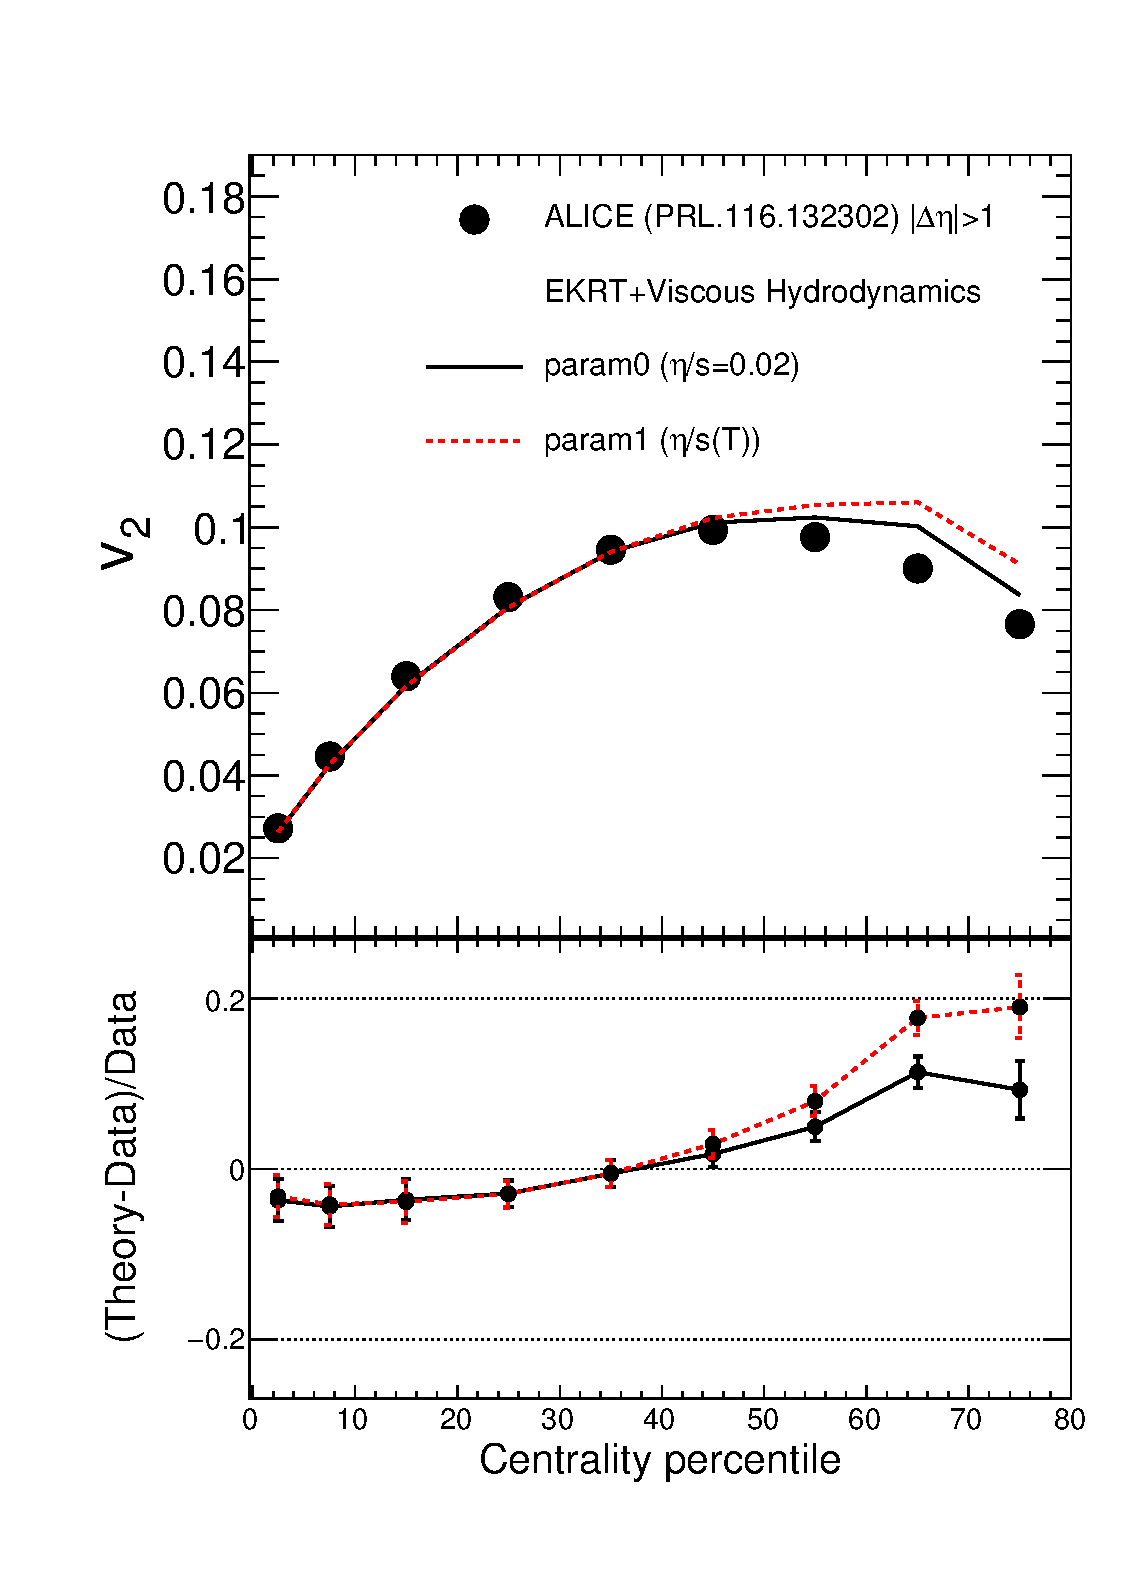
\includegraphics{figs/hydrocom_v2.eps}}
                       \resizebox{0.31\textwidth}{!}{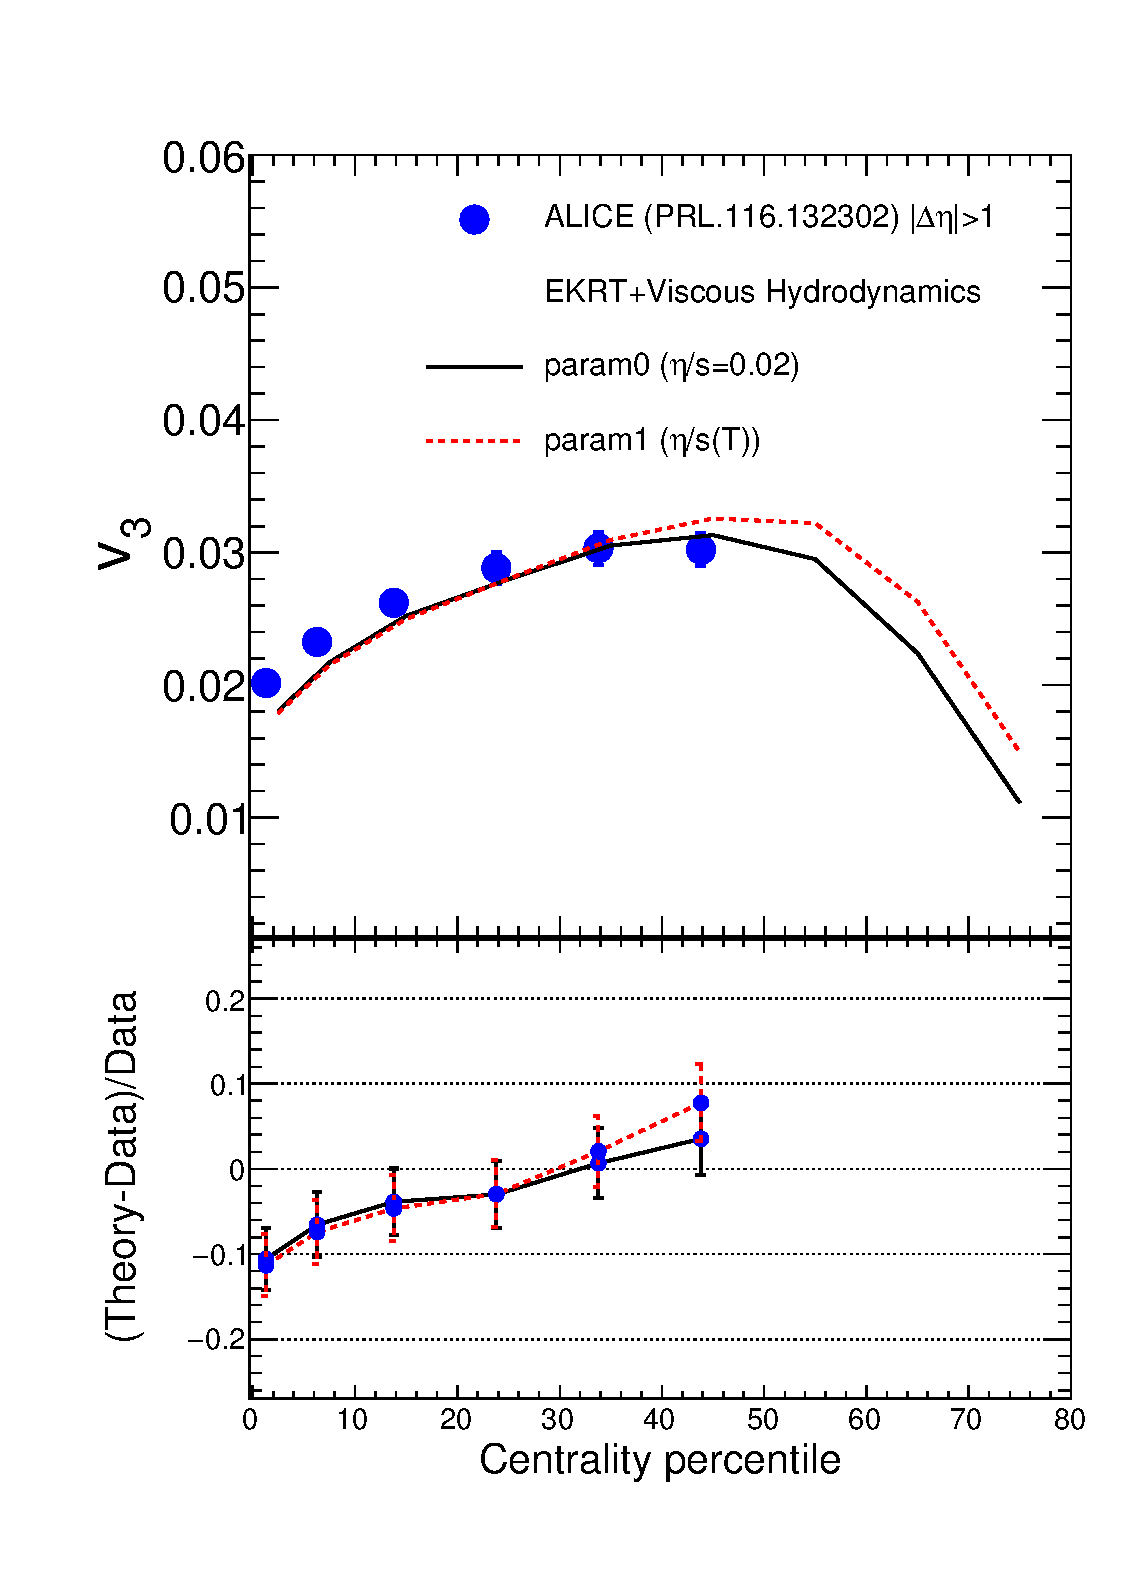
\includegraphics{figs/hydrocom_v3.eps}}
                       \resizebox{0.31\textwidth}{!}{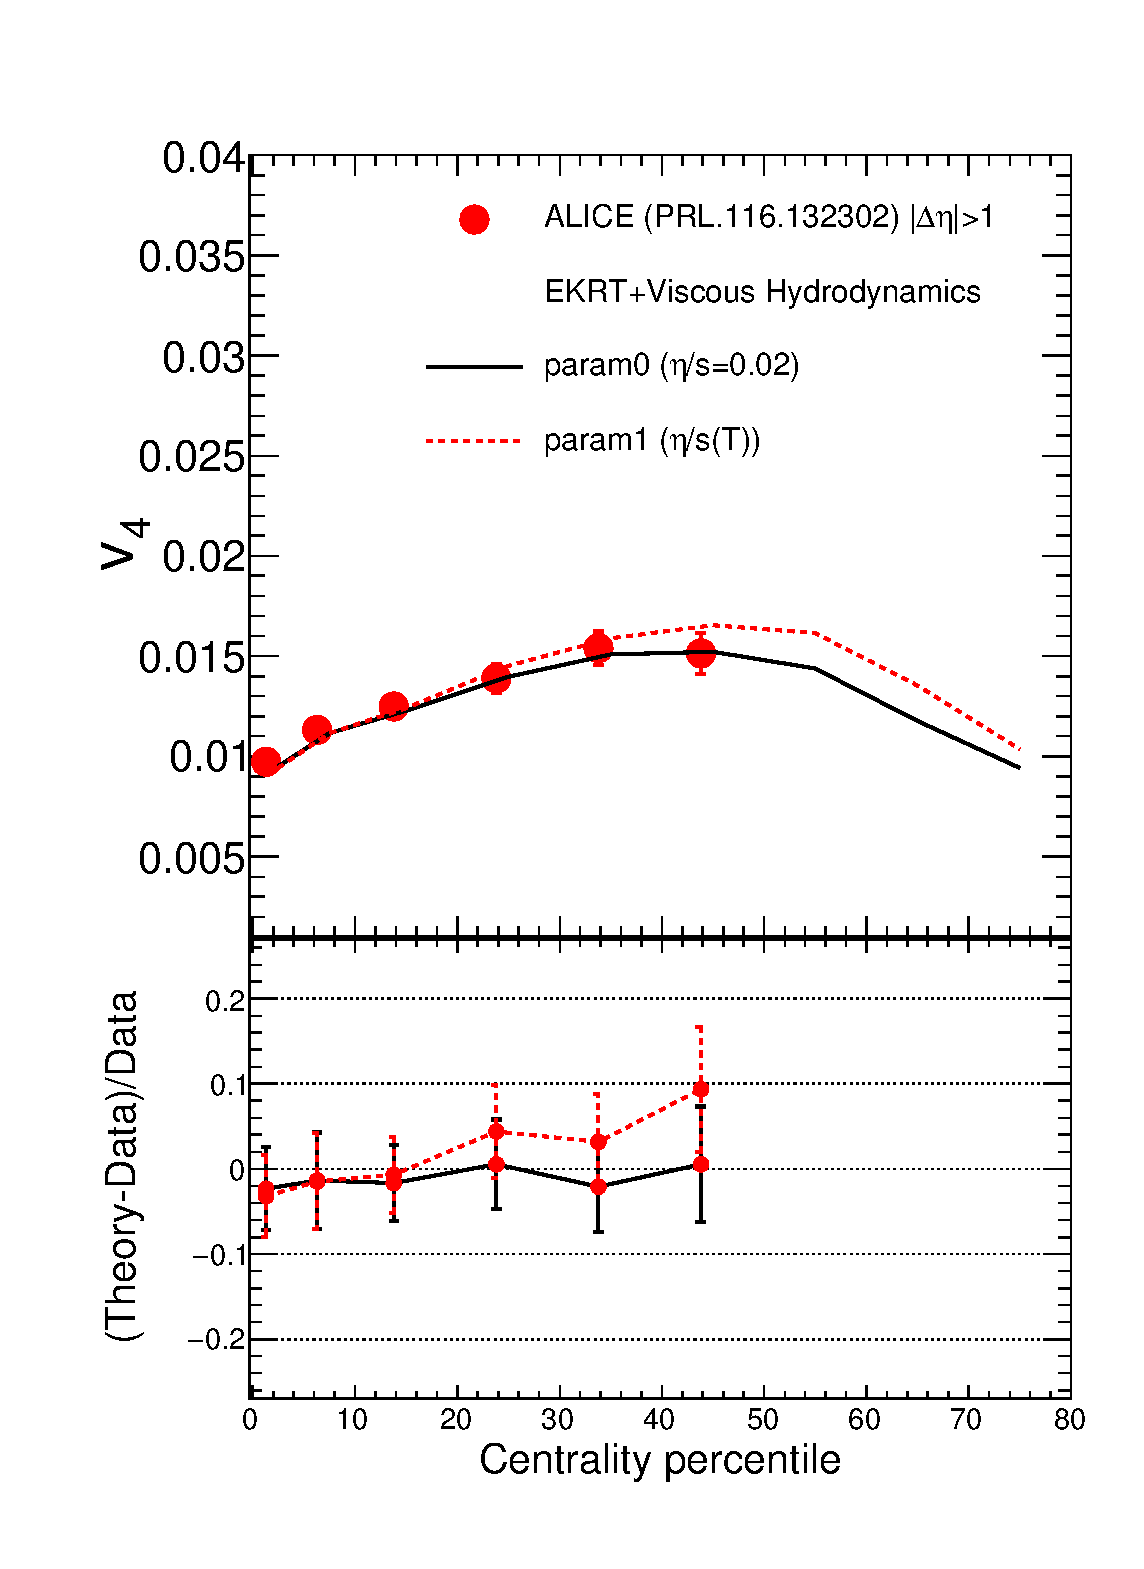
\includegraphics{figs/hydrocom_v4.eps}}
        \caption{The individual flow harmonics $v_n$ (n=2, 3 and 4) in $\PbPb$ collisions at $\snn=2.76$~TeV are compared to the event-by-event EKRT+viscous hydrodynamic calculations~\cite{Niemi:2015qia}. The lines are hydrodynamic predictions with two different $\eta/s(T)$ parameterizations, labeled in the same way as in ~\cite{Niemi:2015qia}.}
        \label{fig:Figure_8}
              \end{center}
\end{figure*}
The event-by-event EKRT+viscous hydrodynamic calculations~\cite{Niemi:2015qia} gives a good description of the charged hadron multiplicity and the low $p_{\rm T}$ region of the charged hadron spectra at RHIC and the LHC (see Figs.~11-13 in \cite{Niemi:2015qia}).
Each of the $\eta/s(T)$ parameterizations is adjusted to reproduce the measured $v_n$ from central to mid-peripheral collisions (see Fig.~15 in \cite{Niemi:2015qia}). 
EKRT The difference to the data is less than 5\% for $v_2$ and 10\% for $v_3$ and $v_4$.
VISH The difference to the data is less than 30\% for $v_2$ and $v_3$,  50\% for $v_4$.
AMPT about 20\% for the default and the string melting version, in case of the string melting version without 

\begin{figure*}[h]
            \begin{center}
                       \resizebox{0.31\textwidth}{!}{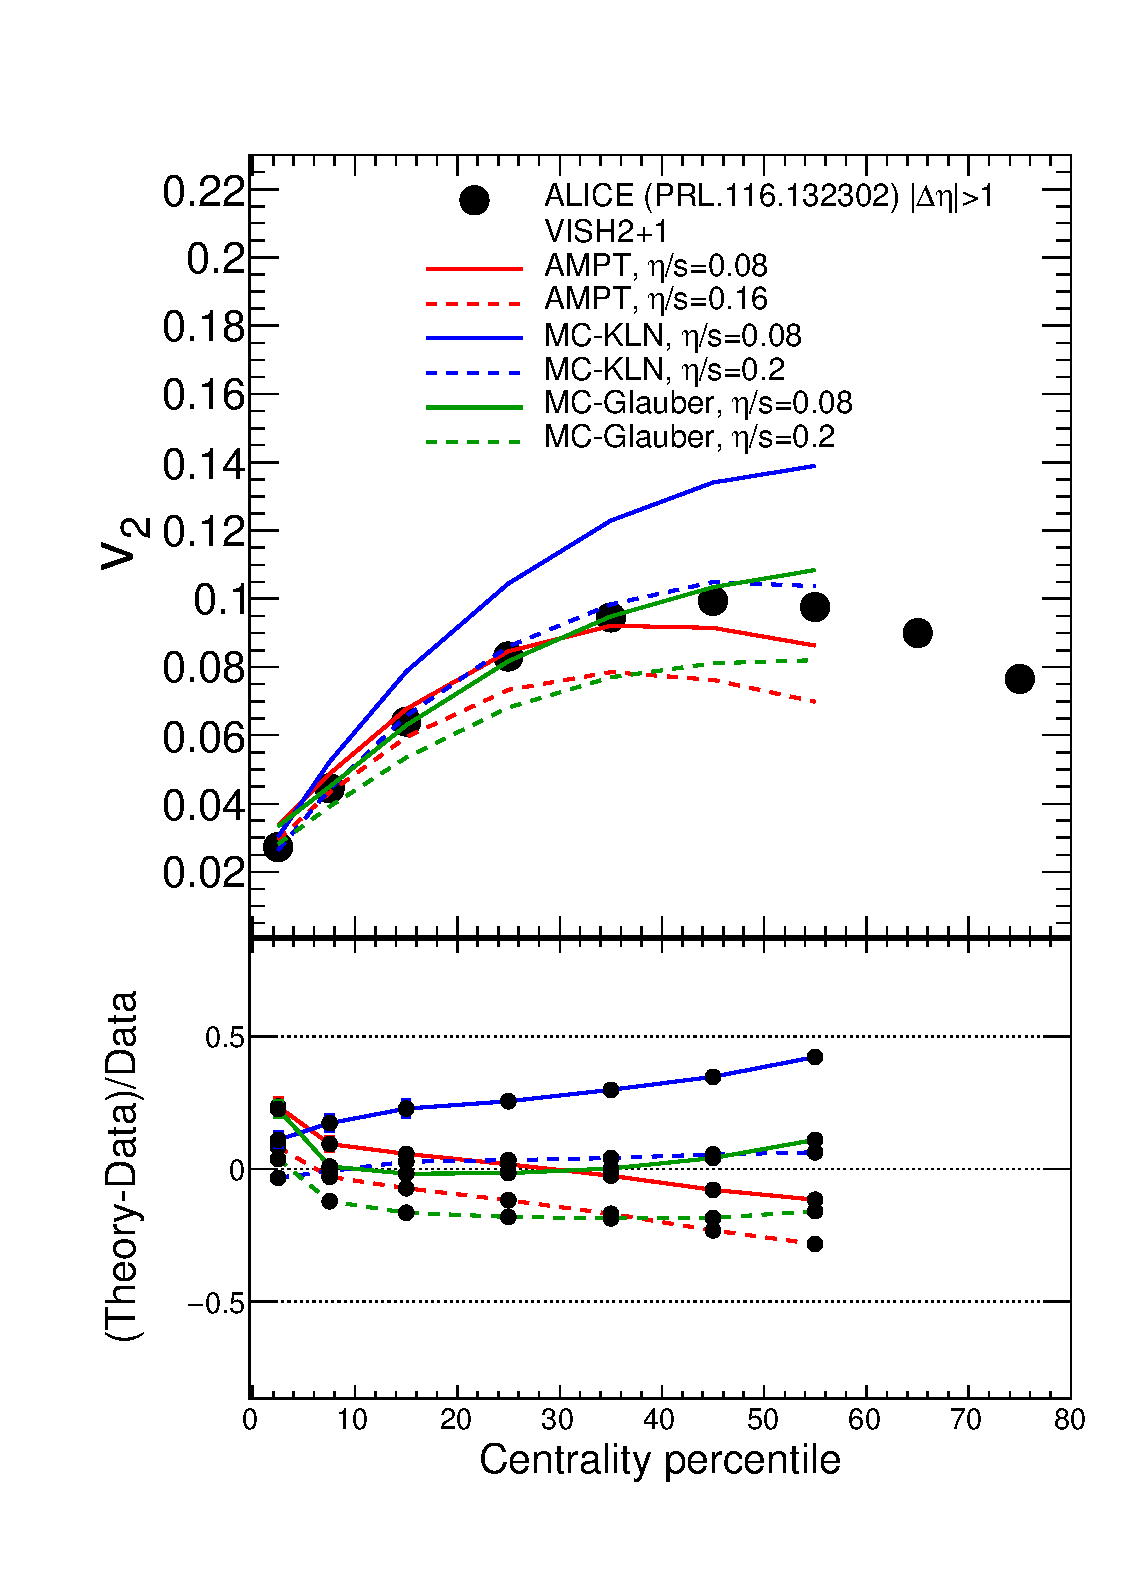
\includegraphics{figs/vishcom_v2.eps}}
                       \resizebox{0.31\textwidth}{!}{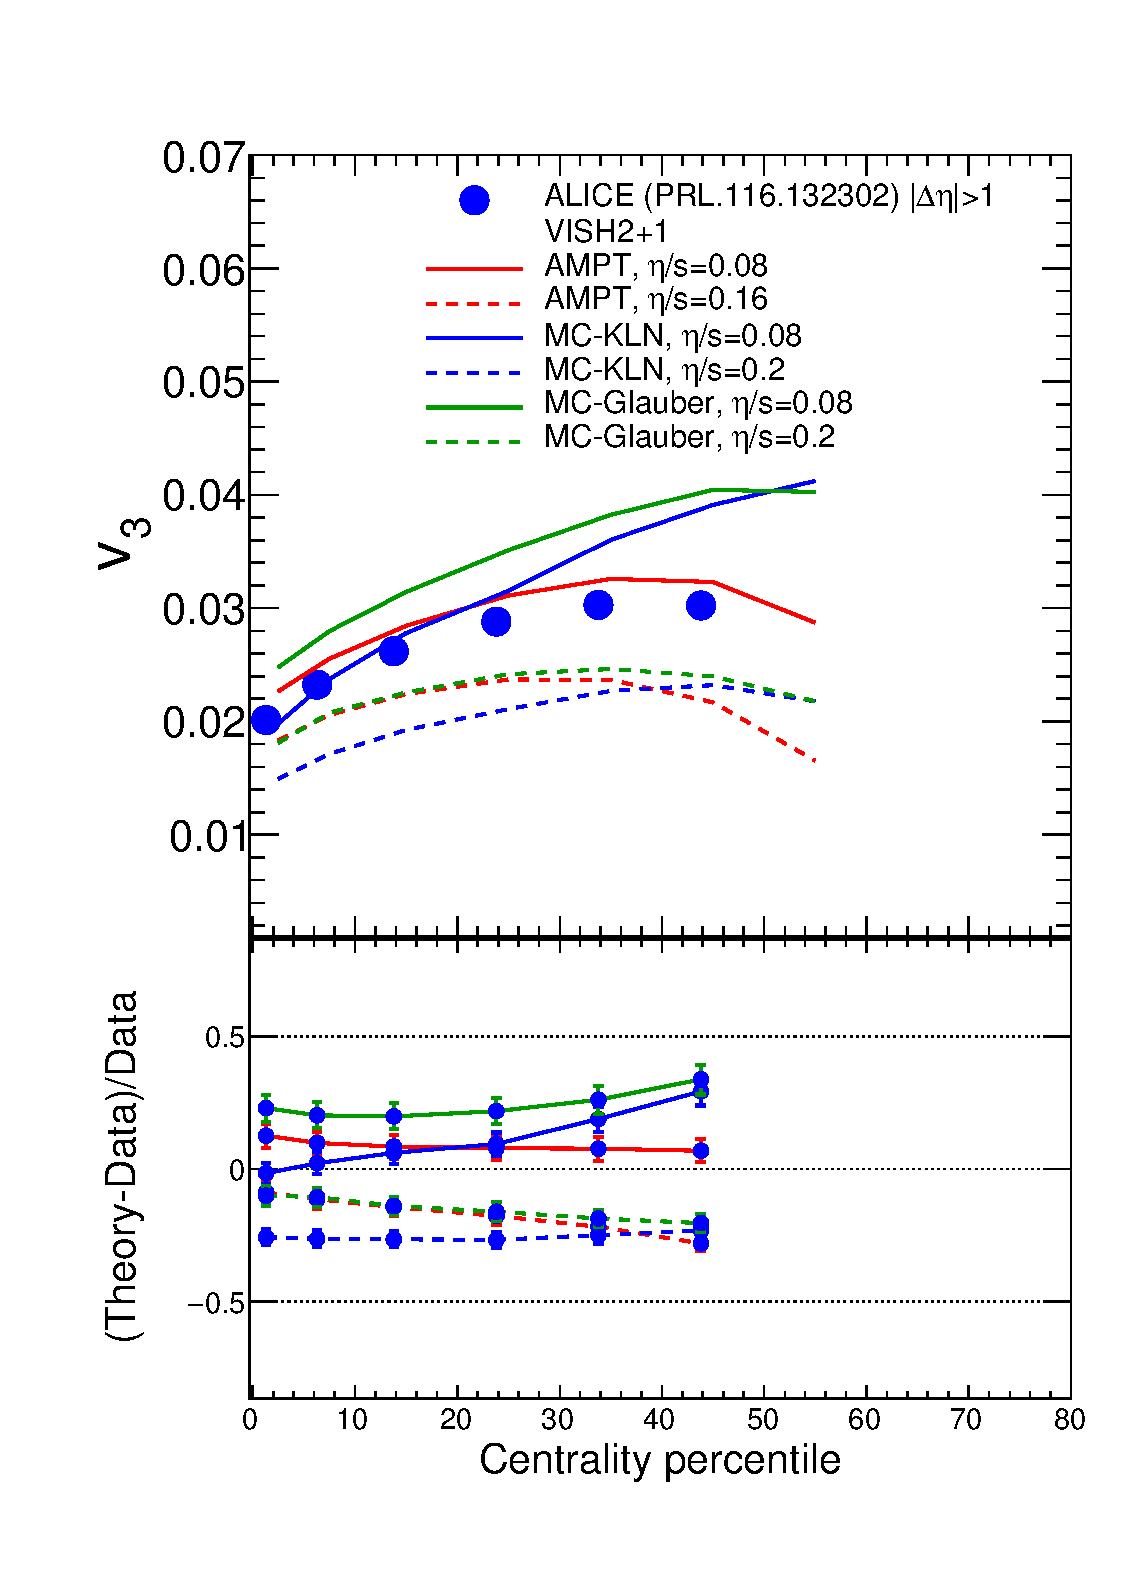
\includegraphics{figs/vishcom_v3.eps}}
                       \resizebox{0.31\textwidth}{!}{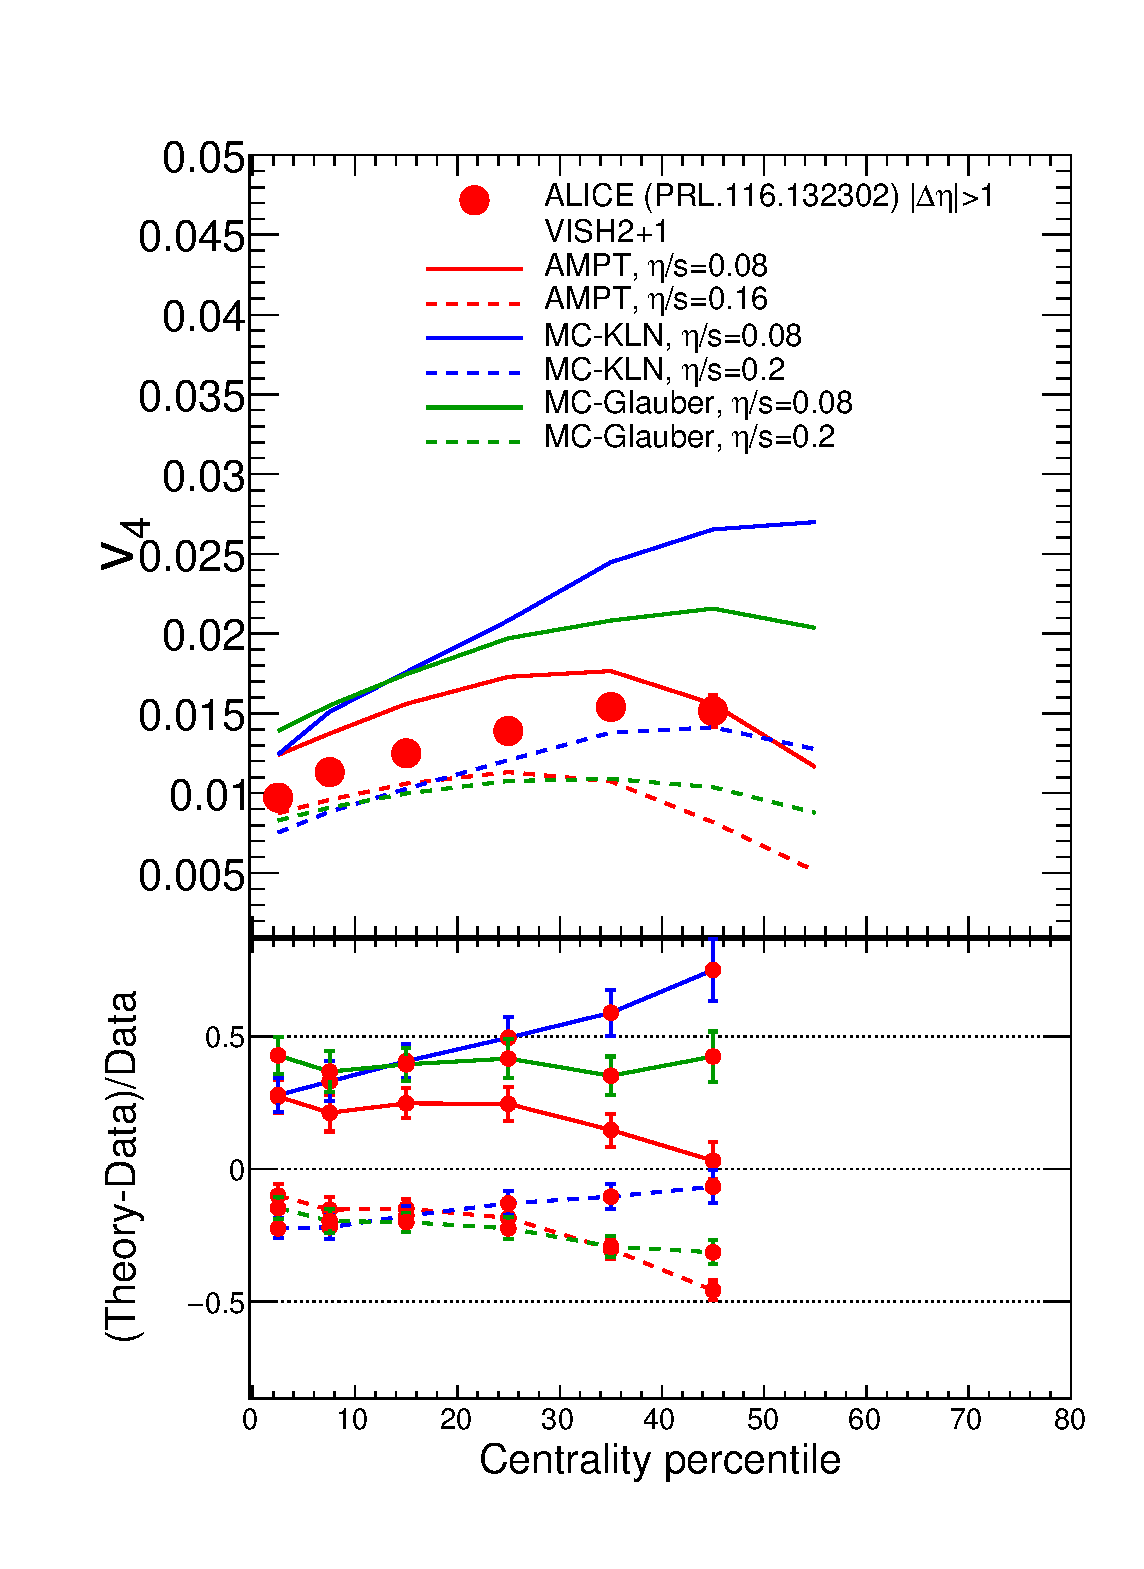
\includegraphics{figs/vishcom_v4.eps}}
        \caption{The individual flow harmonics $v_n$ (n=2, 3 and 4) in $\PbPb$ collisions at $\snn=2.76$~TeV are compared to various VISH2+1 calculations~\cite{Zhu:2016puf}. Three initial conditions from AMPT, MC-KLN and MC-Glauber are drawn as different colors and markers. The $\eta/s$ parameters are shown as different line styles, the small shear viscosity ($\eta/s=0.08$) are shown as solid lines, and large shear viscosities ($\eta/s=0.2$ for MC-KLN and MC-Glauber, 0.16 for AMPT) are drawn as dashed lines.}
        \label{fig:Figure_9}
              \end{center}
\end{figure*}

%neither MC-Glauber nor MC-KLN initial con- ditions can simultaneously describe v2, v3, and v4, as once reported in [41]. More specifically, for MC-Glauber initial conditions, VISH2+1 with η/s = 0.08 could nicely fit the integrated v2 from central to semi-peripheral col- lisions, but overestimates v3 and v4 for the same central- ity classes. For MC-KLN initial conditions, VISH2+1 with η/s = 0.20 reproduces the integrated flow v2 but under- estimates v3 and v4 for the presented centrality classes. Compared with these two results, hydrodynamic calcu- lations with AMPT initial conditions improves the descrip- tions of vn (n = 2, 3, 4).
Panel (c) shows that VISH2+1 with AMPT initial condition and η/s = 0.08 roughly describe v2, v3 and v4 from central to semi-peripheral collisions.

\begin{figure*}[h]
            \begin{center}
                       \resizebox{0.31\textwidth}{!}{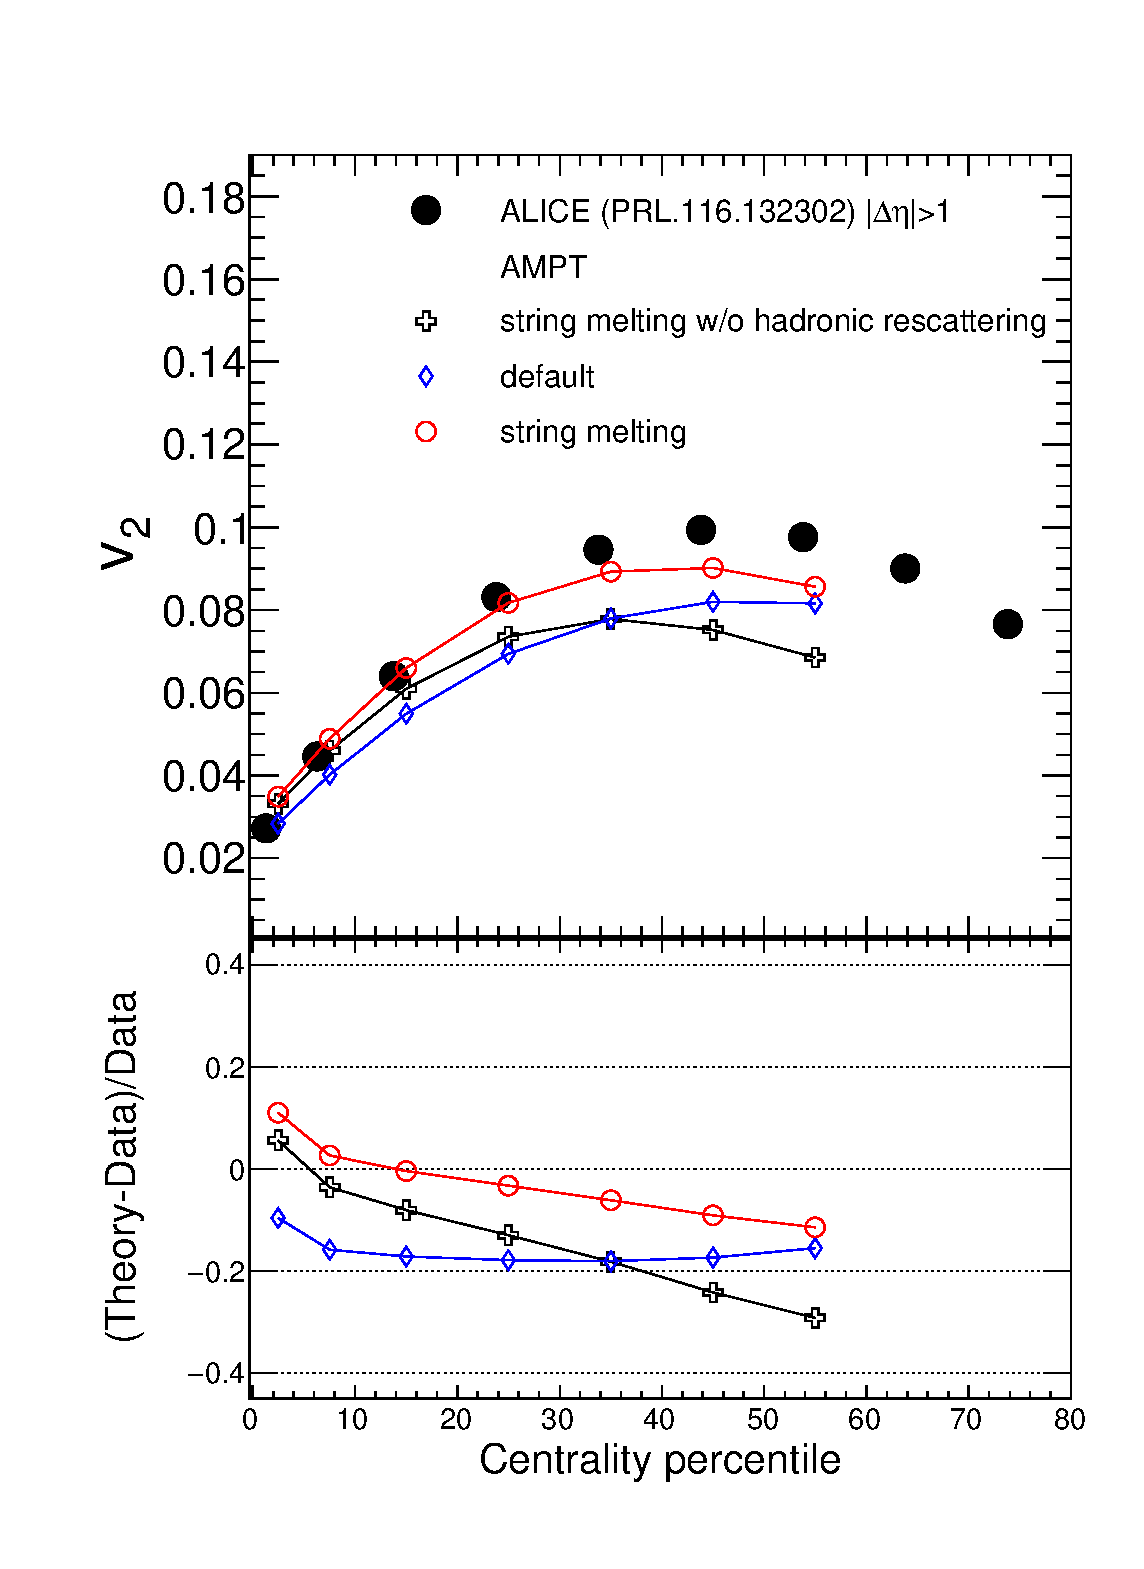
\includegraphics{figs/amptcom_v2.eps}}
                       \resizebox{0.31\textwidth}{!}{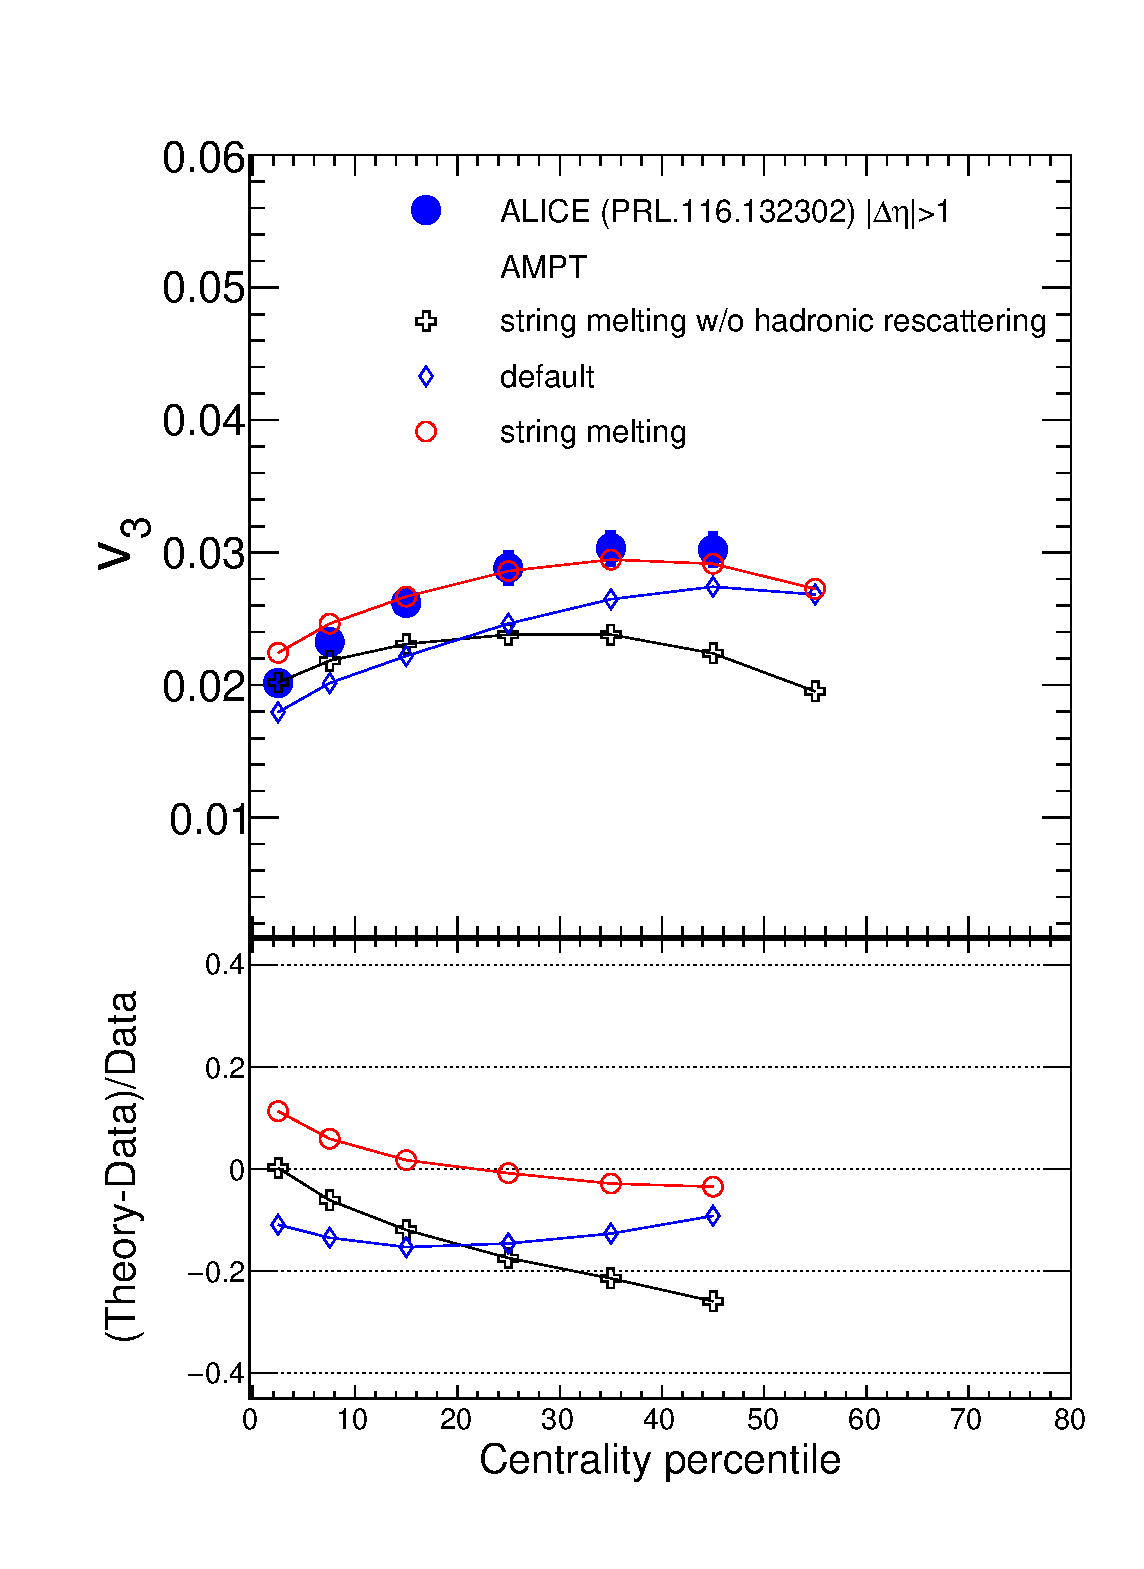
\includegraphics{figs/amptcom_v3.eps}}
                       \resizebox{0.31\textwidth}{!}{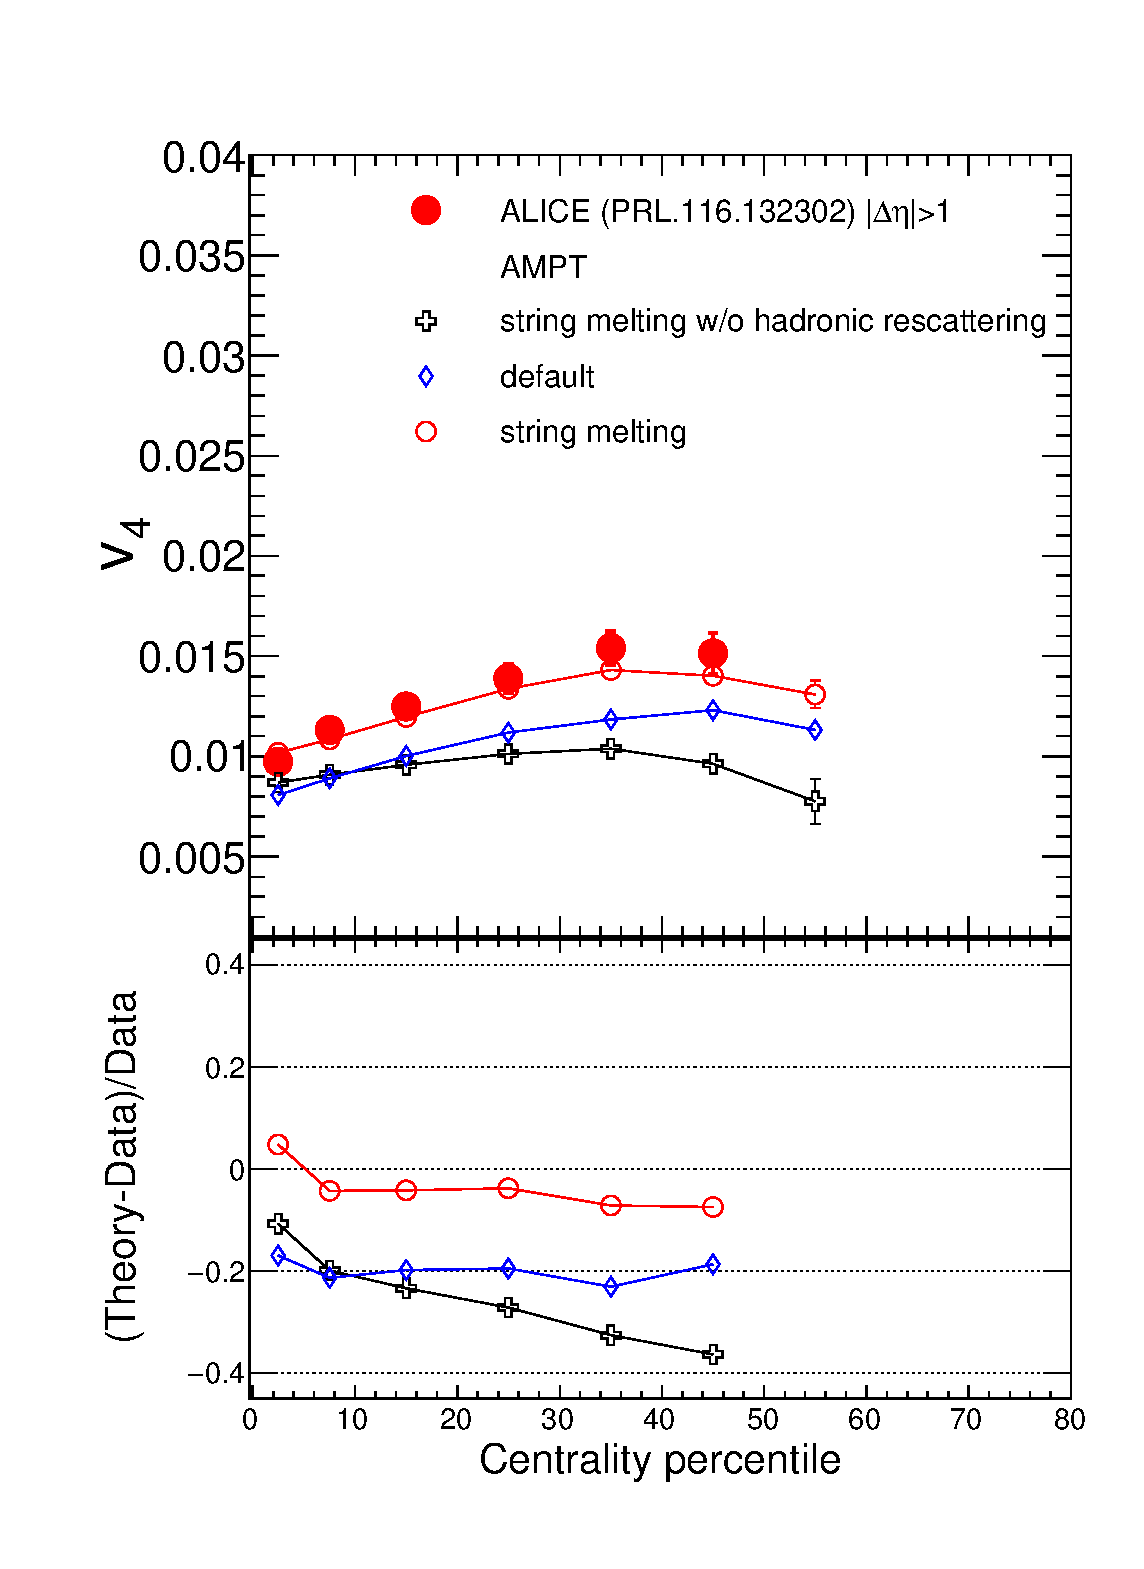
\includegraphics{figs/amptcom_v4.eps}}
        \caption{The individual flow harmonics $v_n$ (n=2, 3 and 4) in $\PbPb$ collisions at $\snn=2.76$~TeV are compared to various AMPT models.}
        \label{fig:Figure_10}
              \end{center}
\end{figure*}

